% siminos/atlas/chart.tex  pdflatex atlas
% $Author$ $Date$

\section{Charting the \reducedsp: Global atlas}
\label{s:chart}

    %
%  \includegraphics[width=1.00\textwidth,clip=true]{slicePhil0}

The \mslices\ as implemented here associates a \slice\ \refeq{PCsectQ0}
to a \template. Our \slice\ is locally a hyperplane, expected to be a
good description of solutions similar to a given template only in its
neighbourhood. Nevertheless, as every group orbit has a point closest to
a given \template, and a \slice\ is the set of all such group-orbit
points, it slices the group orbits of \emph{all} full \statesp\ points.
The variational distance condition \refeq{PCsectQ0} is an extremum
condition, and as the group orbits of highly nonlinear states are highly
contorted (see \reffig{fig:2830GO6}\,{\it b}), the distance function can
have many extrema, and multiple sections by a \slice\ hyperplane. For
example, a \rpo\ sweeps out a torus, and is always intersected by a
\slice\ hyperplane in two or more \po\ sections, once at the orbit's
closest passage to the template, with positive curvature \refeq{eq:curv},
and another time at the most distant passage, also satisfying the slice
condition \refeq{eq:slcond}, but with negative curvature (see
\reffig{fig:sliceimage}\,{\it a}).


    \begin{itemize}
      \item flow in a \slice: \cLf\ example
      \item {\chartBord}: \cLf\ example
      \item 2-chart atlas, ridges:  \cLf\ example
      \item gauge fixing, geometric phase?
    \end{itemize}



%%%%%%%%%%%%%%%%%%%%%%%%%%%%%%%%%%%%%%%%%%%%%%%%%%%%%%%%%%%%%%%%%%%%%
\begin{figure}
   \centering
   %\includegraphics[width=0.45\textwidth]{2841GO3S}
   \caption{\label{fig:sliceimage}
      Every slice hyperplane cuts every group orbit at least twice (see
      \reffig{fig:slice}), once at       orbit's closest passage to the
      {\template}, with positive curvature \refeq{eq:curv},   and another
      time at the most distant passage, also satisfying the slice
      condition \refeq{eq:slcond}, but with negative curvature. An
      $\SOn{2}$ \rpo\ is topologically a torus, so the two cuts are the
      two \po\ images of the same \rpo, the good close one, and the bad
      distant one, on the other side of {\sset}, and thus not in the
      slice. Here this is illustrated by close cut (blue) of the \rpo\
      $\RPO{36.92}$ torus, \reffig{f:MeanVelocityFrame}\,({\it b}),
      plotted together with the most distant cut (red), in the same slice
      hyperplane, but not in the slice.
   }
\end{figure}
%%%%%%%%%%%%%%%%%%%%%%%%%%%%%%%%%%%%%%%%%%%%%%%%%%%%%%%%%%%%%%%%%%%%%

%%%%%%%%%%%%%%%%%%%%%%%%%%%%%%%%%%%%%%%%%%%%%%%%%%%%%%%%%%%%%%%%%%%%%%
%\begin{figure}
%   \centering
%  (a)
%~~(b) 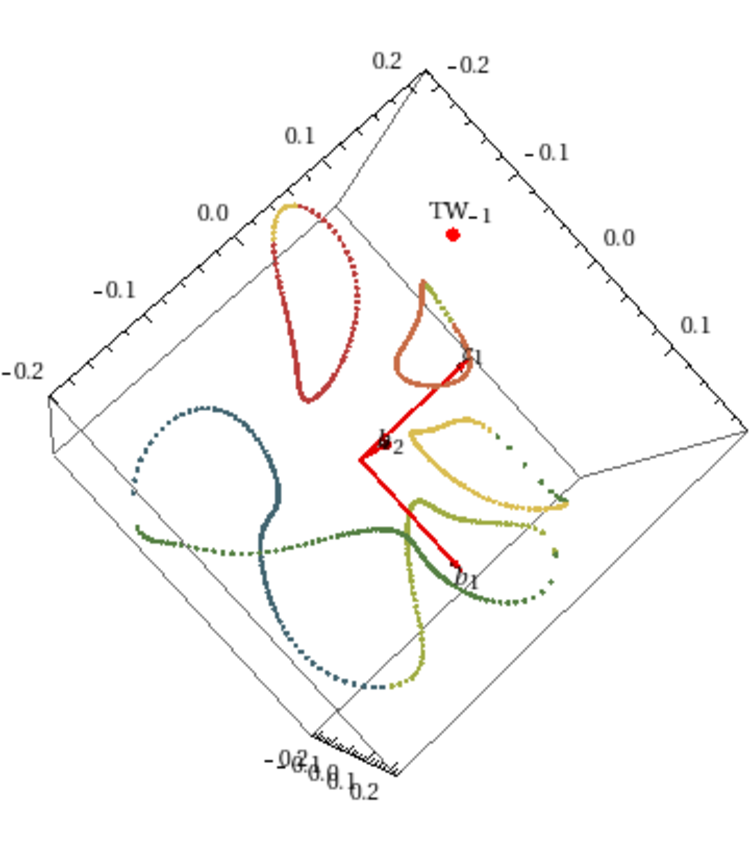
\includegraphics[width=0.45\textwidth]{ks22rpo16mfAll}
%   \caption{ \label{ks22rpo16mf}
%(color online)
%\KS\ \rpo\ with $\period{p}=16.31$, $\shift_p=-2.863$ in a \slice\
%fixed by a \reqv\ \slicep.
%(a)
%(b)
%All intersections of the 2-torus \rpo\ with the \slice\ are plotted.
%Color-coding represents internal numbering of solutions and changes along
%orbits when the number of solutions for $\theta$ changes. We have $3$
%closed-loop images of the \rpo\ and $3$ images that appear to connect to
%a closed loop (from \cite{SiminosThesis}).
%}
%\end{figure}
%%%%%%%%%%%%%%%%%%%%%%%%%%%%%%%%%%%%%%%%%%%%%%%%%%%%%%%%%%%%%%%%%%%%%%




Fortunately, we do have a sharp definition of how far the neighborhood
of a {\template} extends:
a hyperplane captures faithfully neighboring group orbits as long
as it \slice s them transversally; it fails the moment the group tangent of
a not-so close point $\sspRSing$ lies in the \slice.
At this instant the group tangent is orthogonal to the \slice\ tangent,
\beq
\braket{\groupTan(\sspRSing)}{\sliceTan{}}= 0
\, ,
\ee{sspRSing}
%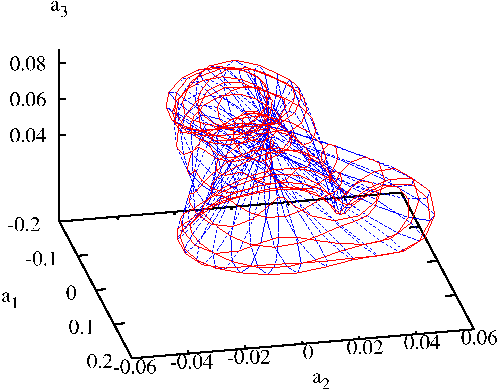
\includegraphics[width=1.20\textwidth]{2840GOt135M1} %{2830GO7}
%  \caption{\label{fig:2830GO6}
    %\label{fig:M1groupOrb}
%
and the phase velocity $\dot{\gSpace}(\sspRSing)$ in \refeq{reconstrEq}
diverges.  For points more distant the group orbits have more than one
intersection with the \slice\ hyperplane. It is clear what the trouble
with any single \slice\ hyperplane is: our slice condition and \slice s
are linear.

The physical task is to, for a given dynamical flow, pick a set of
qualitatively distinct {\template s} (for example, one typical of 2-roll
states, one for 4-roll states, and so on) whose \slice s  are locally
transverse to open sets of nearby orbits, and which together provide a
good global atlas of $\pS/\Group$. Each \slice\ $\pS{}^{(j)}$, provides a
local chart at $\slicep{}^{(j)}$ for a neighborhood of an important,
qualitatively distinct class of solutions. Together they `Voronoi'
tessellate  the curved manifold in which the symmetry-reduced strange
attractor is embedded by a finite set of hyperplane tiles.

Coupled with our \statesp\ visualizations allows for explorations of
high-dimensional flows that hitherto were unthinkable. Symmetry reduction
is here achieved, and now all invariant solutions can be plotted
together, as one happy family: all points equivalent by symmetries are
represented by a single point, families of solutions are mapped to a
single solution, \reqva\ become \eqva, and \rpo s become \po s. Without
symmetry reduction, no full understanding of pipe and plane \pCf s is
possible.
    %
    \PC{2011-10-18 incorporate this paragraph:``
Note also that the rotation of a fluid flow into a \slice\ {\em is not}
an average over the 3D pipe azimuthal angle, it is the full snapshot of
the flow embedded in the $\infty$-dimensional \statesp. Symmetry
reduction is not a dimensional-reduction scheme, or flow modeling by
fewer degrees of freedom: the \reducedsp\ is also $\infty$-dimensional
and no information is lost, one can go freely between solutions in the
full and reduced \statesp s by integrating the associated
\emph{reconstruction equations}.
''}


%%%%%%%%%%%%%%%%%%%%%%%%%%%%%%%%%%%%%%%%%%%%%%%%%%%%%%%%%%%%%%%%
%% A29-2tmplts.* A29-2slices.*: see dasbuch/book/FigSrc/inkscape/00ReadMe.txt
%% Predrag 2012-03-18
%% remember to insert A29-2slices.eps into ChaosBook
 \begin{figure}
 \begin{center}
  \setlength{\unitlength}{0.40\textwidth}
  %% \unitlength = units used in the Picture Environment
(a)
  \begin{picture}(1,0.58916866)%
    \put(0,0){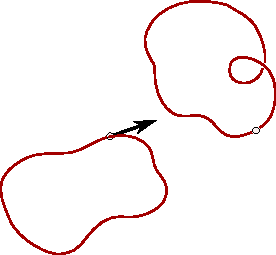
\includegraphics[width=\unitlength]{A29-2tmplts}}%
    \put(0.28946003,0.42825178){\color[rgb]{0,0,0}\makebox(0,0)[lb]{\smash{$\slicep{}^{(1)}$}}}%
    \put(0.65414286,0.29589463){\color[rgb]{0,0,0}\makebox(0,0)[lb]{\smash{$\hat{\slicep{}}^{(2)}$}}}%
    \put(0.48952418,0.46705018){\color[rgb]{0,0,0}\makebox(0,0)[lb]{\smash{$\sliceTan{}{}^{(1)}$}}}%
    \put(0.70483139,0.50323639){\color[rgb]{0,0,0}\makebox(0,0)[lb]{\smash{$\sliceTan{}{}^{(2)}$}}}%
    \put(0.88901848,0.05071544){\color[rgb]{0,0,0}\makebox(0,0)[lb]{\smash{$\slicep{}^{(2)}$}}}%
  \end{picture}%
\\
(b)
{\small
  \begin{picture}(1,0.5520358)%
    \put(0,0){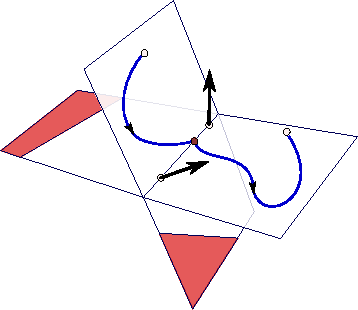
\includegraphics[width=\unitlength]{A29-2slices}}%
    \put(0.56508945,0.42521319){\color[rgb]{0,0,0}\makebox(0,0)[lb]{\smash{$(1)$}}}%
    \put(0.9511718,0.42521319){\color[rgb]{0,0,0}\makebox(0,0)[lb]{\smash{$(2)$}}}%
    \put(0.22307502,0.24294119){\color[rgb]{0,0,0}\makebox(0,0)[lb]{\smash{$\slicep{}^{(1)}$}}}%
    \put(0.3997654,0.18632793){\color[rgb]{0,0,0}\makebox(0,0)[lb]{\smash{$\hat{\slicep{}}^{(2)}$}}}%
    \put(0.23319206,0.43234865){\color[rgb]{0,0,0}\rotatebox{-52.7950691}{\makebox(0,0)[lb]{\smash{$(1)$}}}}%
    \put(0.46613918,0.23896304){\color[rgb]{0,0,0}\rotatebox{-13.98154984}{\makebox(0,0)[lb]{\smash{$(2)$}}}}%
    \put(0.11710635,0.24747479){\color[rgb]{0,0,0}\makebox(0,0)[lb]{\smash{$\sspRed(0)$}}}%
    \put(0.30171828,0.37769283){\color[rgb]{0,0,0}\makebox(0,0)[lb]{\smash{$\sspRed(\zeit)$}}}%
    \put(0.56508945,0.22594488){\color[rgb]{0,0,0}\makebox(0,0)[lb]{\smash{$(3)$}}}%
    \put(0.57577014,0.29987052){\color[rgb]{0,0,0}\makebox(0,0)[lb]{\smash{$\sspRed(0)$}}}%
    \put(0.63404136,0.4168711){\color[rgb]{0,0,0}\makebox(0,0)[lb]{\smash{$\sspRed(\zeit)$}}}%
    \put(0.89513496,0.40380004){\color[rgb]{0,0,0}\makebox(0,0)[lb]{\smash{$\slicep{}^{(1)}$}}}%
    \put(0.70083156,0.35473521){\color[rgb]{0,0,0}\makebox(0,0)[lb]{\smash{$\hat{\slicep{}}^{(2)}$}}}%
  \end{picture}%
} % end {\small
 \end{center}
 \caption{\label{fig:A29-2slices}
A 2-chart atlas.
(a)
Start with the {\template} $\slicep{}^{(1)}$. All group orbits traverse
its slice hyperplane, including the group orbit of the neighboring
{\template} $\slicep{}^{(2)}$. Replace this {\template} by its closest
group-orbit point $\hat{\slicep{}}^{(2)}$, \ie, the point in \slice\
$\pSRed{}^{(1)}$.
(b)
As these two points are the closest group orbit points, they lies in the
slice of each \template. However, the two tangent vectors
$\sliceTan{}{}^{(1)}$ and $\sliceTan{}{}^{(2)}$ have different
orientations, so they define two distinct \slice\ hyperplanes
$\pSRed{}^{(1)}$ and $\pSRed{}^{(2)}$ which intersect in a ridge; the
chart for the neighborhood of each template (a page of the atlas on the
right side of the figure) extends only as far as this ridge. If the
templates are sufficiently close, the {\chartBord} of each \slice\ (red
region) is beyond this ridge, and never encountered by the
symmetry-reduced trajectory $\sspRed(\zeit)$. The reduced trajectory is
continuous in the slice comprised of such charts - it switches the chart
whenever it crosses a ridge common to a pair of charts.
 }
 \end{figure}
%%%%%%%%%%%%%%%%%%%%%%%%%%%%%%%%%%%%%%%%%%%%%%%%%%%%%%%%%%%%%%%%


\subsection{Global atlas}
% Predrag 2012-03-04: transferred here text from slice.tex

A \slice\ hyperplane captures faithfully neighboring group orbits until,
for a point $\sspRSing$ not so close to the \template\ its tangent vector
lies in the \slice,
\[
\braket{\groupTan(\sspRSing)}{\sliceTan{}}= 0
\,,
\]
and its group orbit is grazed tangentially rather than sliced transversally.
The {\phaseVel} $\dot{\gSpace}(\sspRSing)$ in
\refeq{reconstrEq} then diverges. Equivalently,
one can say that a \slice\ is transverse to a group orbit as long as its
curvature normal vector \refeq{eq:curv} is not normal to the {\template} vector,
\[
\braket{\groupTan(\sspSing)}{\sliceTan{}}
 =
-\braket{\Lg^2\sspSing}{\slicep}
 =
-\braket{\kappa(\sspSing) \,{\bf n}(\sspSing)}{\slicep}
 = 0
\,.
\]
This is also a linear condition, and it defines a hyperplane of points
\sspSing\ normal to  the quadratic Casimir-weighted curvature vector
$\kappa(\slicep) \, {\bf n}(\slicep)$, such that from the {\template} vantage
point their group orbits are not transverse, but locally `horizontal.'
%$(d\!-\!2)$\dmn\
{\Sset} $S$ is the locus of inflection points, a hyperplane through which
curvature of the distance function changes sign:
    \PC{demonstrate this}
set of all points
$\sspRSing$ which are both in the {\slice}, and whose group tangent
$\groupTan(\sspRSing)$ is also in the  {\slice},
    \PC{add Froehlich figure of {\Sset} $S$?}
    % 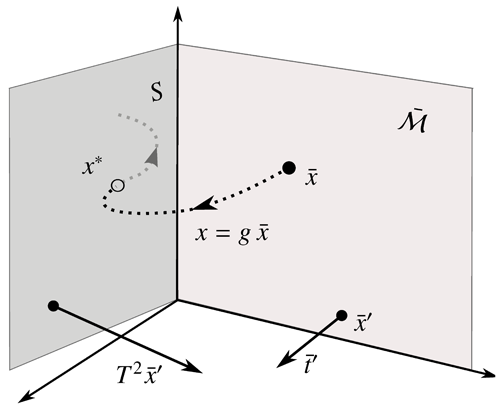
\includegraphics[width=0.80\textwidth]{inflectHype.png}
\beq
\braket{\sspRSing}{\sliceTan{}} \,=\, 0
    \,, \mbox{ and }
\braket{\groupTan(\sspRSing)}{\sliceTan{}}
 \,=\,
-\braket{\sspRSing}{\kappa(\slicep) \, {n}(\slicep)}
 =0
\,.
\label{sliceSingl0}
\eeq
A hyperplane segment of a \slice\ is good only up to the \sset. However,
the divergence in {\phaseVel} \refeq{reconstrEq} is an artifact of the
symmetry reduction by tangent hyperplanes, and thus an avoidable
nuisance.

Locally, our initial \slice\ chart $\pSRed{}^{(1)}$ is a ($d\!-\!1$)\dmn\
hyperplane. If we pick another {\template} point $\slicep{}^{(2)}$, it
comes along with its own \slice\ hyperplane $\pSRed{}^{(2)}$. Any
neighboring pair of $(d\!-\!1)$\dmn\ local \slice\ hyperplanes intersects
in a `ridge',
% (`boundary,' `edge'),
a $(d\!-\!2)$\dmn\ hyperplane, easy to compute.

Once templates are picked, the rest is geometry of hyperplanes (nothing
to do with dynamics, only with the group theory) so checking whether the
inflection hyperplane is on the far side of the ridge between two \slice
s is a linear computation, to be undertaken independently of dynamics.
For a reduced trajectory moving in $\pSRed{}^{(1)}$ one only has to keep checking
the sign of
\[
\braket{(\sspRed(\zeit)- \hat{\slicep{}}^{(2)})}{\sliceTan{}{}^{(2)}}
\,.
\]
Once this changes the sign, the ridge has been crossed, and from then on the
trajectory should be reduced to the $\pSRed{}^{(2)}$ slice. There is no need to
pinpoint this crossing accurately, as long $\sspRed(\zeit)$ stays well clear of
all \chartBord s.

Thus, in order to chart the \statesp\ of a chaotic flow, a set
of local \slice\ hyperplanes is needed to capture all of the asymptotic
dynamics. The choice of local \slice s should reflect the dynamically
dominant patterns seen in the solutions of nonlinear PDEs. We construct a
global atlas of the dimensionally \reducedsp\ $\pSRed = \pS/\Group$ by
deploying local linear \slice s  $\pS{}^{(j)}$ across neighborhoods of
the qualitatively most important \template\ {\cohStr s}
$\slicep{}^{(j)}$. For example, in reducing chaotic trajectories of
\refsect{s:rpos}, we use a set of \reqva\ as our \template s, see
\reffig{fig:thetadot2}. This is the periodic-orbit implementation of the
idea of {\statesp\ tessellation}.

The physical task is to, for a given dynamical flow, pick a set of
qualitatively distinct {\template s} whose \slice s  are locally
transverse to an open set of nearby orbits. Each \slice\ $\pS{}^{(j)}$,
provides a local chart at $\slicep{}^{(j)}$ for a neighborhood of an
important, qualitatively distinct class of solutions (2-rolls states,
3-rolls states, \etc). Together they `Voronoi' tessellate  the curved
manifold in which the symmetry-reduced strange attractor is embedded by a
finite set of hyperplane tiles. We have no advice on how to
systematically pick the individual \template s, other than that the
associated \slice\ tiles should be sufficiently small to exclude
group-orbit tangencies, \ie, stop before crossing their inflection
hyperplanes \refeq{sliceSingl0}.

    \ifdraft\color{blue}
``The origin'' or the invariant, fixed-point subspace is a
high-dimensional center space of points not moved by $\Lg_{\theta}$. For
\pCf\ it is the space plumbers prefer to compute in, even though all
turbulence is in the full \statesp. The reason why I really, really want
us to understand what is going on with our atlas in \reffig{fig:A29-2slices}
is that the singularities might be genuine, due to close passages to this
center space, and not taken care of by $\sspRSing$ (which all also
include the `origin'), not just due to bad choice of \template s.
    \color{black}\fi

    \begin{itemize}
      \item an atlas is \emph{not needed} for Newton determination of a
            single orbit; any local section and slice plus time and shift
            constraints is OK, can even move them with each Newton
            iteration. 60,000 \rpo s can be computed\rf{SCD07} this way.
            The question is: what then? and for that you need a good atlas.
    \end{itemize}
